\subsection{Herausforderungen}
Hier sind besonders erwähnenswerte Herausforderungen und Hürden beschrieben, die sich im Verlaufe des Projektes gestellt haben. Dies soll anderen Software Ingenieuren oder Interessierten helfen  aus unseren Schwierigkeiten zu lernen. 

\subsubsection{HTTPS REST Schnittstelle in CI/CD aufsetzen}
Während dem Entwickeln des Prototyps in der Evaluation stellten wir fest, dass das Abfragen unserer Backend-Schnittstelle auf Android wie gewünscht funktionierte, jedoch warf die Applikation beim Ausführen auf iOS eine Exception. Der Grund dafür war, dass iOS keine Verbindungen zu unverschlüsselten Webseiten mehr zulässt. Daher war der Fall klar, dass dies noch aufgesetzt werden muss.

Nach kurzen Recherchen haben wir für das Erstellen und Validieren des Zertifikates auf Let's Encrypt \cite{letsencrypt} gewählt, gerade deshalb weil eine ausführliche Dokumentation und eine rasche Generierung möglich ist. 

Auch mit dem verwendeten Play Framework sollte das Aufsetzen der HTTPS Site kein Problem darstellen, es sollte mit einem Parameter beim Start der Applikation gut möglich sein. 

Nachdem das Zertifikat installiert wurde und die Applikation lokal erfolgreich lief, galt es, das Gesamte noch in den Build-Prozess einzubauen. Dabei kam das Problem auf, dass der Pfad zum Keystore, der das Let's Encrypt-Zertifikat beinhaltet, nicht gültig war. Nach mehrmaligem, gründlichem Überprüfen des Pfades und neu Builden, wurden immer noch Exceptions geworfen.

Wir haben keinen Anhaltspunkt, was der Fehler sein könnte, denn werden die genau gleichen Befehle auf dem Backend-Server direkt ausgeführt, funktioniert die Applikation einwandfrei auf HTTPS. Sobald es aber über den Build-Server läuft, findet er den Pfad zum Keystore nicht mehr.

Als Work-Around haben wir eine \texttt{CustomSslEngineProvider} geschrieben, der den Pfad zum Keystore direkt im Code beinhaltet. Darauf hat Puppet keinen Einfluss und die Applikation funktioniert wie gewünscht.

\subsubsection{Kritisches Design der Brainstorming Logik im Frontend}
Im Verlaufe der Entwicklungsphasen hat sich insbesondere die Klasse \texttt{Brain\-storming\-PageViewModel} stetig vergrössert und wurde komplexer. Die gesamte Logik für den Blattwechsel, das Holen der verbleibenden Zeit, das Ein- und Ausblenden einiger Controls sowie das Überprüfen, ob eine Runde abgeschlossen wurde, ist in dieser Klasse implementiert. 

Wie wir bald feststellten, macht eine solche Klasse die Fehlersuche sehr schwierig. Es wurden zwar einige kleinere Bugs behoben, aber es wurden dabei auch neue aufgedeckt beziehungsweise eingeschleust. Wenn zwei Timers aktiv sind und somit Parallelität im Spiel ist, ist das Verhalten der App nicht deterministisch. So haben wir die Situation, dass einmal eine Runde einwandfrei funktioniert, und ein andermal mit derselben Konfiguration die Controls nicht richtig aktualisiert werden. 

Um die Komplexität zu verringern, wurde ein Konzept erarbeitet, welches in einer allfälligen Folgearbeit umgesetzt werden sollte. Dabei geht es darum, eine State-Machine einzuführen, welche die drei Zustände \textbf{Waiting}, \textbf{Running} und \textbf{Ended} enthält. Bei jedem Aufruf der ViewModel-Klasse wird zu Beginn überprüft, in welchem Zustand das aktuelle Finding ist und die Maschine wird dann in den entsprechenden Zustand versetzt. Darauf sind alle für die Controls benötigten Properties und Timers implementiert. 

Der grosse Vorteil bei dieser Lösung ist, dass der Überblick zurückgewonnen werden kann und somit eine sauberere Fehlerbehandlung möglich ist. Auch Erweiterungen sind somit einfacher möglich (zum Beispiel Hinzufügen eines "Review"-States). 

Abbildung \ref{fig:statemachine-brainstorming} erklärt das Konzept anhand einem Zustandsdiagramm.
\begin{figure}
	\centering
	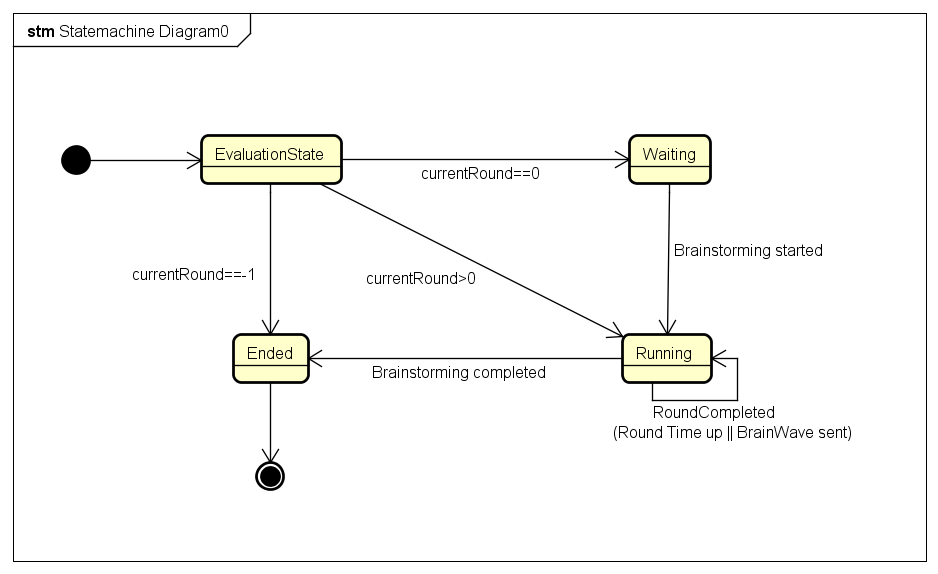
\includegraphics[width=0.7\linewidth]{img/techn-bericht/statemachine-brainstorming}
	\caption{Zustandsmaschine für Brainstorminglogik}
	\label{fig:statemachine-brainstorming}
\end{figure}

\paragraph*{Workaround}
Als aktuelle Lösung bieten wir ein Sync-Button an, der beim Betätigen die Brainstorming Page aktualisiert. Dies hat zur Folge, dass alle Daten vom Backend geholt und wieder gesetzt werden. Wenn zum Beispiel ein Rundenwechsel nicht funktioniert hat, eignet sich dieses Feature, um den korrekten Zustand wiederherzustellen und mit dem Backend zu synchronisieren. Der Button ist im Icon hinterlegt, wie in Abbildung \ref{fig:sync-workaround} sichtbar.

\begin{figure}
	\centering
	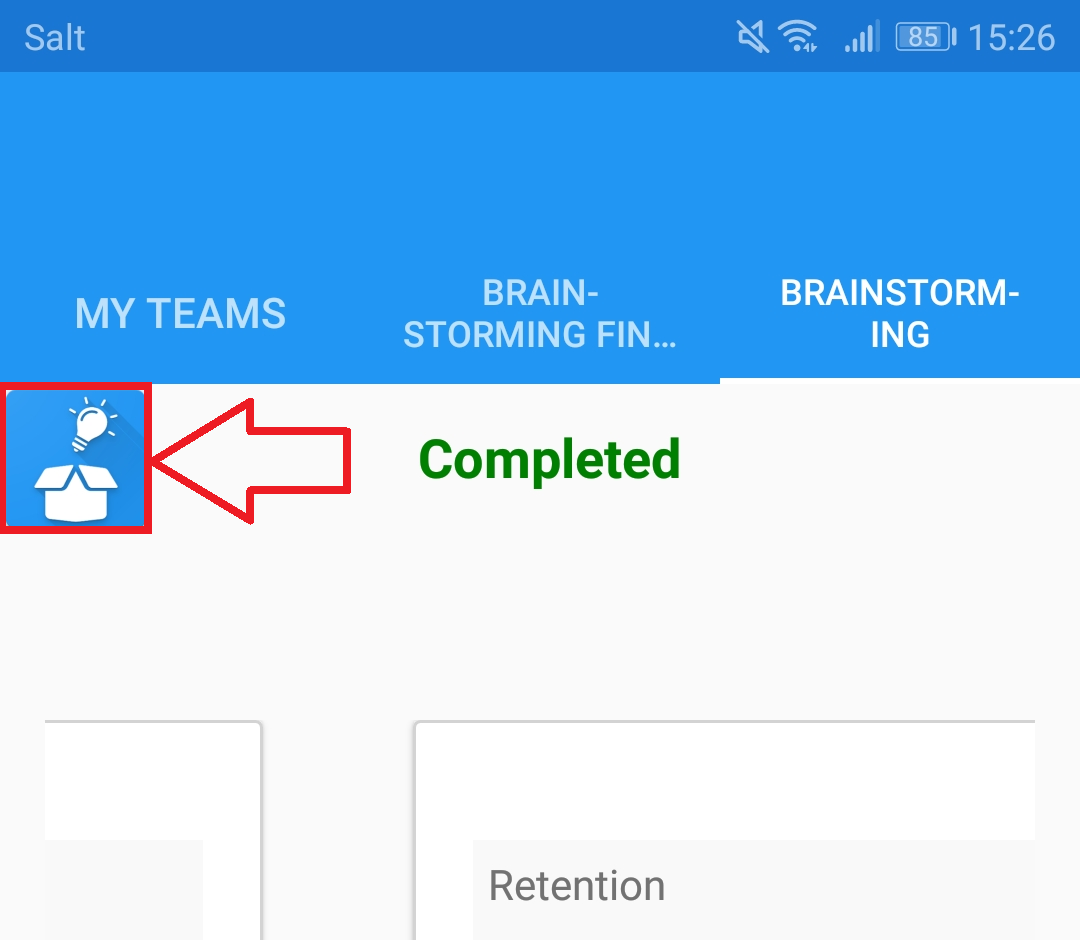
\includegraphics[width=0.35\linewidth]{img/techn-bericht/sync-workaround}
	\caption{Sync Button}
	\label{fig:sync-workaround}
\end{figure}

